\documentclass[11pt,a4paper]{article}

% shared/macros.tex
% Shared notation for all surface-partition math documents.
% Include with: % shared/macros.tex
% Shared notation for all surface-partition math documents.
% Include with: % shared/macros.tex
% Shared notation for all surface-partition math documents.
% Include with: \input{../shared/macros}

% -------------------------------------------------------------------------
% Packages (include here so each document only needs \input{../shared/macros})
% -------------------------------------------------------------------------
\usepackage{amsmath,amssymb,amsthm}
\usepackage{bm}           % \bm for bold math
\usepackage{mathtools}    % \coloneqq, dcases, etc.
\usepackage{booktabs}     % \toprule etc. in tables
\usepackage{hyperref}
\usepackage{geometry}
\usepackage{microtype}
\usepackage{parskip}
\usepackage{xcolor}
\usepackage{tcolorbox}
\usepackage{enumitem}
\usepackage{float}             % [H] float placement

\geometry{a4paper, margin=2.5cm}

% -------------------------------------------------------------------------
% Theorem-like environments
% -------------------------------------------------------------------------
\theoremstyle{definition}
\newtheorem{defn}{Definition}[section]
\newtheorem{remark}{Remark}[section]

\theoremstyle{plain}
\newtheorem{prop}{Proposition}[section]

% -------------------------------------------------------------------------
% Mesh and geometry
% -------------------------------------------------------------------------
\newcommand{\V}{\mathbf{V}}            % vertex array V[i] in R^dim
\newcommand{\F}{\mathbf{F}}            % face (triangle) array
\newcommand{\vone}[1]{v_{1,#1}}       % first vertex index of VP i
\newcommand{\vtwo}[1]{v_{2,#1}}       % second vertex index of VP i

% -------------------------------------------------------------------------
% Variable points
% -------------------------------------------------------------------------
\newcommand{\lam}{\lambda}             % scalar VP parameter
\newcommand{\Lam}{\boldsymbol{\lambda}}% full parameter vector
\newcommand{\vp}[1]{\mathbf{p}_{#1}}  % 3D position of VP i
\newcommand{\ed}[1]{\mathbf{d}_{#1}}  % edge direction d_i = V[v1_i] - V[v2_i]

% -------------------------------------------------------------------------
% Steiner / triple-point
% -------------------------------------------------------------------------
\newcommand{\Sv}{\mathbf{S}}           % Steiner (Fermat-Torricelli) point
\newcommand{\Ki}{K_{i}}               % projection matrix (I-n_i n_i^T)/r_i
\newcommand{\Mmat}{M}                 % sum of K_i matrices at a triple point

% -------------------------------------------------------------------------
% Normals and unit vectors
% -------------------------------------------------------------------------
\newcommand{\nhat}{\hat{\mathbf{n}}}  % unit normal to a triangle
\newcommand{\Dhat}{\hat{\boldsymbol{\Delta}}}  % unit segment direction

% -------------------------------------------------------------------------
% Operations
% -------------------------------------------------------------------------
\newcommand{\norm}[1]{\left\|#1\right\|}
\newcommand{\abs}[1]{\left|#1\right|}
\newcommand{\ip}[2]{\langle #1,\, #2 \rangle}

% Projection perpendicular to a unit vector \uhat
\newcommand{\Proj}[1]{\bigl(\mathbf{I} - #1 #1^\top\bigr)}

% argmax operator (winner-take-all assignment in Phase 1 documents)
\DeclareMathOperator*{\argmax}{arg\,max}
\DeclareMathOperator*{\argmin}{arg\,min}

% -------------------------------------------------------------------------
% Calculus shorthands
% -------------------------------------------------------------------------
\newcommand{\pd}[2]{\dfrac{\partial #1}{\partial #2}}
\newcommand{\pdd}[3]{\dfrac{\partial^2 #1}{\partial #2\,\partial #3}}
\newcommand{\grad}{\nabla}
\newcommand{\Hess}[1]{\nabla^2 #1}

% -------------------------------------------------------------------------
% Optimization problem objects
% -------------------------------------------------------------------------
\newcommand{\Preg}{P_{\mathrm{reg}}}  % regular perimeter
\newcommand{\Pst}{P_{\mathrm{st}}}   % Steiner perimeter
\newcommand{\Areg}{A^{\mathrm{reg}}} % regular cell area
\newcommand{\Ast}{A^{\mathrm{st}}}   % Steiner area contribution
\newcommand{\Atgt}{\bar{A}}           % target area per cell
\newcommand{\Lagr}{\mathcal{L}}       % Lagrangian
\newcommand{\objfac}{\sigma}          % IPOPT objective scaling factor

% -------------------------------------------------------------------------
% Code cross-references (for "In the code..." callouts)
% -------------------------------------------------------------------------
\newcommand{\code}[1]{\texttt{#1}}
\newcommand{\codefile}[1]{\texttt{\small #1}}

% -------------------------------------------------------------------------
% Threshold dynamics / approach B (10-mbo-auction-dynamics)
% -------------------------------------------------------------------------
\newcommand{\Dlump}{D}                 % lumped mass matrix diag(v)
\newcommand{\Atau}{A_\tau}             % discrete diffusion operator (M + tau K)^{-1} M
\newcommand{\Etau}{E_\tau}             % heat-content (threshold-dynamics) energy
\newcommand{\Rcell}{R_{\mathrm{cell}}} % radius of the equal-area disc sqrt(Abar/pi)
\newcommand{\hmean}{h_{\mathrm{mean}}} % mean edge length
\newcommand{\hmax}{h_{\mathrm{max}}}   % max edge length
\newcommand{\Gt}{G_t}                  % heat kernel at time t
\newcommand{\Ktau}{K^{\mathrm{res}}_\tau} % resolvent (backward-Euler) kernel


% -------------------------------------------------------------------------
% Packages (include here so each document only needs % shared/macros.tex
% Shared notation for all surface-partition math documents.
% Include with: \input{../shared/macros}

% -------------------------------------------------------------------------
% Packages (include here so each document only needs \input{../shared/macros})
% -------------------------------------------------------------------------
\usepackage{amsmath,amssymb,amsthm}
\usepackage{bm}           % \bm for bold math
\usepackage{mathtools}    % \coloneqq, dcases, etc.
\usepackage{booktabs}     % \toprule etc. in tables
\usepackage{hyperref}
\usepackage{geometry}
\usepackage{microtype}
\usepackage{parskip}
\usepackage{xcolor}
\usepackage{tcolorbox}
\usepackage{enumitem}
\usepackage{float}             % [H] float placement

\geometry{a4paper, margin=2.5cm}

% -------------------------------------------------------------------------
% Theorem-like environments
% -------------------------------------------------------------------------
\theoremstyle{definition}
\newtheorem{defn}{Definition}[section]
\newtheorem{remark}{Remark}[section]

\theoremstyle{plain}
\newtheorem{prop}{Proposition}[section]

% -------------------------------------------------------------------------
% Mesh and geometry
% -------------------------------------------------------------------------
\newcommand{\V}{\mathbf{V}}            % vertex array V[i] in R^dim
\newcommand{\F}{\mathbf{F}}            % face (triangle) array
\newcommand{\vone}[1]{v_{1,#1}}       % first vertex index of VP i
\newcommand{\vtwo}[1]{v_{2,#1}}       % second vertex index of VP i

% -------------------------------------------------------------------------
% Variable points
% -------------------------------------------------------------------------
\newcommand{\lam}{\lambda}             % scalar VP parameter
\newcommand{\Lam}{\boldsymbol{\lambda}}% full parameter vector
\newcommand{\vp}[1]{\mathbf{p}_{#1}}  % 3D position of VP i
\newcommand{\ed}[1]{\mathbf{d}_{#1}}  % edge direction d_i = V[v1_i] - V[v2_i]

% -------------------------------------------------------------------------
% Steiner / triple-point
% -------------------------------------------------------------------------
\newcommand{\Sv}{\mathbf{S}}           % Steiner (Fermat-Torricelli) point
\newcommand{\Ki}{K_{i}}               % projection matrix (I-n_i n_i^T)/r_i
\newcommand{\Mmat}{M}                 % sum of K_i matrices at a triple point

% -------------------------------------------------------------------------
% Normals and unit vectors
% -------------------------------------------------------------------------
\newcommand{\nhat}{\hat{\mathbf{n}}}  % unit normal to a triangle
\newcommand{\Dhat}{\hat{\boldsymbol{\Delta}}}  % unit segment direction

% -------------------------------------------------------------------------
% Operations
% -------------------------------------------------------------------------
\newcommand{\norm}[1]{\left\|#1\right\|}
\newcommand{\abs}[1]{\left|#1\right|}
\newcommand{\ip}[2]{\langle #1,\, #2 \rangle}

% Projection perpendicular to a unit vector \uhat
\newcommand{\Proj}[1]{\bigl(\mathbf{I} - #1 #1^\top\bigr)}

% argmax operator (winner-take-all assignment in Phase 1 documents)
\DeclareMathOperator*{\argmax}{arg\,max}
\DeclareMathOperator*{\argmin}{arg\,min}

% -------------------------------------------------------------------------
% Calculus shorthands
% -------------------------------------------------------------------------
\newcommand{\pd}[2]{\dfrac{\partial #1}{\partial #2}}
\newcommand{\pdd}[3]{\dfrac{\partial^2 #1}{\partial #2\,\partial #3}}
\newcommand{\grad}{\nabla}
\newcommand{\Hess}[1]{\nabla^2 #1}

% -------------------------------------------------------------------------
% Optimization problem objects
% -------------------------------------------------------------------------
\newcommand{\Preg}{P_{\mathrm{reg}}}  % regular perimeter
\newcommand{\Pst}{P_{\mathrm{st}}}   % Steiner perimeter
\newcommand{\Areg}{A^{\mathrm{reg}}} % regular cell area
\newcommand{\Ast}{A^{\mathrm{st}}}   % Steiner area contribution
\newcommand{\Atgt}{\bar{A}}           % target area per cell
\newcommand{\Lagr}{\mathcal{L}}       % Lagrangian
\newcommand{\objfac}{\sigma}          % IPOPT objective scaling factor

% -------------------------------------------------------------------------
% Code cross-references (for "In the code..." callouts)
% -------------------------------------------------------------------------
\newcommand{\code}[1]{\texttt{#1}}
\newcommand{\codefile}[1]{\texttt{\small #1}}

% -------------------------------------------------------------------------
% Threshold dynamics / approach B (10-mbo-auction-dynamics)
% -------------------------------------------------------------------------
\newcommand{\Dlump}{D}                 % lumped mass matrix diag(v)
\newcommand{\Atau}{A_\tau}             % discrete diffusion operator (M + tau K)^{-1} M
\newcommand{\Etau}{E_\tau}             % heat-content (threshold-dynamics) energy
\newcommand{\Rcell}{R_{\mathrm{cell}}} % radius of the equal-area disc sqrt(Abar/pi)
\newcommand{\hmean}{h_{\mathrm{mean}}} % mean edge length
\newcommand{\hmax}{h_{\mathrm{max}}}   % max edge length
\newcommand{\Gt}{G_t}                  % heat kernel at time t
\newcommand{\Ktau}{K^{\mathrm{res}}_\tau} % resolvent (backward-Euler) kernel
)
% -------------------------------------------------------------------------
\usepackage{amsmath,amssymb,amsthm}
\usepackage{bm}           % \bm for bold math
\usepackage{mathtools}    % \coloneqq, dcases, etc.
\usepackage{booktabs}     % \toprule etc. in tables
\usepackage{hyperref}
\usepackage{geometry}
\usepackage{microtype}
\usepackage{parskip}
\usepackage{xcolor}
\usepackage{tcolorbox}
\usepackage{enumitem}
\usepackage{float}             % [H] float placement

\geometry{a4paper, margin=2.5cm}

% -------------------------------------------------------------------------
% Theorem-like environments
% -------------------------------------------------------------------------
\theoremstyle{definition}
\newtheorem{defn}{Definition}[section]
\newtheorem{remark}{Remark}[section]

\theoremstyle{plain}
\newtheorem{prop}{Proposition}[section]

% -------------------------------------------------------------------------
% Mesh and geometry
% -------------------------------------------------------------------------
\newcommand{\V}{\mathbf{V}}            % vertex array V[i] in R^dim
\newcommand{\F}{\mathbf{F}}            % face (triangle) array
\newcommand{\vone}[1]{v_{1,#1}}       % first vertex index of VP i
\newcommand{\vtwo}[1]{v_{2,#1}}       % second vertex index of VP i

% -------------------------------------------------------------------------
% Variable points
% -------------------------------------------------------------------------
\newcommand{\lam}{\lambda}             % scalar VP parameter
\newcommand{\Lam}{\boldsymbol{\lambda}}% full parameter vector
\newcommand{\vp}[1]{\mathbf{p}_{#1}}  % 3D position of VP i
\newcommand{\ed}[1]{\mathbf{d}_{#1}}  % edge direction d_i = V[v1_i] - V[v2_i]

% -------------------------------------------------------------------------
% Steiner / triple-point
% -------------------------------------------------------------------------
\newcommand{\Sv}{\mathbf{S}}           % Steiner (Fermat-Torricelli) point
\newcommand{\Ki}{K_{i}}               % projection matrix (I-n_i n_i^T)/r_i
\newcommand{\Mmat}{M}                 % sum of K_i matrices at a triple point

% -------------------------------------------------------------------------
% Normals and unit vectors
% -------------------------------------------------------------------------
\newcommand{\nhat}{\hat{\mathbf{n}}}  % unit normal to a triangle
\newcommand{\Dhat}{\hat{\boldsymbol{\Delta}}}  % unit segment direction

% -------------------------------------------------------------------------
% Operations
% -------------------------------------------------------------------------
\newcommand{\norm}[1]{\left\|#1\right\|}
\newcommand{\abs}[1]{\left|#1\right|}
\newcommand{\ip}[2]{\langle #1,\, #2 \rangle}

% Projection perpendicular to a unit vector \uhat
\newcommand{\Proj}[1]{\bigl(\mathbf{I} - #1 #1^\top\bigr)}

% argmax operator (winner-take-all assignment in Phase 1 documents)
\DeclareMathOperator*{\argmax}{arg\,max}
\DeclareMathOperator*{\argmin}{arg\,min}

% -------------------------------------------------------------------------
% Calculus shorthands
% -------------------------------------------------------------------------
\newcommand{\pd}[2]{\dfrac{\partial #1}{\partial #2}}
\newcommand{\pdd}[3]{\dfrac{\partial^2 #1}{\partial #2\,\partial #3}}
\newcommand{\grad}{\nabla}
\newcommand{\Hess}[1]{\nabla^2 #1}

% -------------------------------------------------------------------------
% Optimization problem objects
% -------------------------------------------------------------------------
\newcommand{\Preg}{P_{\mathrm{reg}}}  % regular perimeter
\newcommand{\Pst}{P_{\mathrm{st}}}   % Steiner perimeter
\newcommand{\Areg}{A^{\mathrm{reg}}} % regular cell area
\newcommand{\Ast}{A^{\mathrm{st}}}   % Steiner area contribution
\newcommand{\Atgt}{\bar{A}}           % target area per cell
\newcommand{\Lagr}{\mathcal{L}}       % Lagrangian
\newcommand{\objfac}{\sigma}          % IPOPT objective scaling factor

% -------------------------------------------------------------------------
% Code cross-references (for "In the code..." callouts)
% -------------------------------------------------------------------------
\newcommand{\code}[1]{\texttt{#1}}
\newcommand{\codefile}[1]{\texttt{\small #1}}

% -------------------------------------------------------------------------
% Threshold dynamics / approach B (10-mbo-auction-dynamics)
% -------------------------------------------------------------------------
\newcommand{\Dlump}{D}                 % lumped mass matrix diag(v)
\newcommand{\Atau}{A_\tau}             % discrete diffusion operator (M + tau K)^{-1} M
\newcommand{\Etau}{E_\tau}             % heat-content (threshold-dynamics) energy
\newcommand{\Rcell}{R_{\mathrm{cell}}} % radius of the equal-area disc sqrt(Abar/pi)
\newcommand{\hmean}{h_{\mathrm{mean}}} % mean edge length
\newcommand{\hmax}{h_{\mathrm{max}}}   % max edge length
\newcommand{\Gt}{G_t}                  % heat kernel at time t
\newcommand{\Ktau}{K^{\mathrm{res}}_\tau} % resolvent (backward-Euler) kernel


% -------------------------------------------------------------------------
% Packages (include here so each document only needs % shared/macros.tex
% Shared notation for all surface-partition math documents.
% Include with: % shared/macros.tex
% Shared notation for all surface-partition math documents.
% Include with: \input{../shared/macros}

% -------------------------------------------------------------------------
% Packages (include here so each document only needs \input{../shared/macros})
% -------------------------------------------------------------------------
\usepackage{amsmath,amssymb,amsthm}
\usepackage{bm}           % \bm for bold math
\usepackage{mathtools}    % \coloneqq, dcases, etc.
\usepackage{booktabs}     % \toprule etc. in tables
\usepackage{hyperref}
\usepackage{geometry}
\usepackage{microtype}
\usepackage{parskip}
\usepackage{xcolor}
\usepackage{tcolorbox}
\usepackage{enumitem}
\usepackage{float}             % [H] float placement

\geometry{a4paper, margin=2.5cm}

% -------------------------------------------------------------------------
% Theorem-like environments
% -------------------------------------------------------------------------
\theoremstyle{definition}
\newtheorem{defn}{Definition}[section]
\newtheorem{remark}{Remark}[section]

\theoremstyle{plain}
\newtheorem{prop}{Proposition}[section]

% -------------------------------------------------------------------------
% Mesh and geometry
% -------------------------------------------------------------------------
\newcommand{\V}{\mathbf{V}}            % vertex array V[i] in R^dim
\newcommand{\F}{\mathbf{F}}            % face (triangle) array
\newcommand{\vone}[1]{v_{1,#1}}       % first vertex index of VP i
\newcommand{\vtwo}[1]{v_{2,#1}}       % second vertex index of VP i

% -------------------------------------------------------------------------
% Variable points
% -------------------------------------------------------------------------
\newcommand{\lam}{\lambda}             % scalar VP parameter
\newcommand{\Lam}{\boldsymbol{\lambda}}% full parameter vector
\newcommand{\vp}[1]{\mathbf{p}_{#1}}  % 3D position of VP i
\newcommand{\ed}[1]{\mathbf{d}_{#1}}  % edge direction d_i = V[v1_i] - V[v2_i]

% -------------------------------------------------------------------------
% Steiner / triple-point
% -------------------------------------------------------------------------
\newcommand{\Sv}{\mathbf{S}}           % Steiner (Fermat-Torricelli) point
\newcommand{\Ki}{K_{i}}               % projection matrix (I-n_i n_i^T)/r_i
\newcommand{\Mmat}{M}                 % sum of K_i matrices at a triple point

% -------------------------------------------------------------------------
% Normals and unit vectors
% -------------------------------------------------------------------------
\newcommand{\nhat}{\hat{\mathbf{n}}}  % unit normal to a triangle
\newcommand{\Dhat}{\hat{\boldsymbol{\Delta}}}  % unit segment direction

% -------------------------------------------------------------------------
% Operations
% -------------------------------------------------------------------------
\newcommand{\norm}[1]{\left\|#1\right\|}
\newcommand{\abs}[1]{\left|#1\right|}
\newcommand{\ip}[2]{\langle #1,\, #2 \rangle}

% Projection perpendicular to a unit vector \uhat
\newcommand{\Proj}[1]{\bigl(\mathbf{I} - #1 #1^\top\bigr)}

% argmax operator (winner-take-all assignment in Phase 1 documents)
\DeclareMathOperator*{\argmax}{arg\,max}
\DeclareMathOperator*{\argmin}{arg\,min}

% -------------------------------------------------------------------------
% Calculus shorthands
% -------------------------------------------------------------------------
\newcommand{\pd}[2]{\dfrac{\partial #1}{\partial #2}}
\newcommand{\pdd}[3]{\dfrac{\partial^2 #1}{\partial #2\,\partial #3}}
\newcommand{\grad}{\nabla}
\newcommand{\Hess}[1]{\nabla^2 #1}

% -------------------------------------------------------------------------
% Optimization problem objects
% -------------------------------------------------------------------------
\newcommand{\Preg}{P_{\mathrm{reg}}}  % regular perimeter
\newcommand{\Pst}{P_{\mathrm{st}}}   % Steiner perimeter
\newcommand{\Areg}{A^{\mathrm{reg}}} % regular cell area
\newcommand{\Ast}{A^{\mathrm{st}}}   % Steiner area contribution
\newcommand{\Atgt}{\bar{A}}           % target area per cell
\newcommand{\Lagr}{\mathcal{L}}       % Lagrangian
\newcommand{\objfac}{\sigma}          % IPOPT objective scaling factor

% -------------------------------------------------------------------------
% Code cross-references (for "In the code..." callouts)
% -------------------------------------------------------------------------
\newcommand{\code}[1]{\texttt{#1}}
\newcommand{\codefile}[1]{\texttt{\small #1}}

% -------------------------------------------------------------------------
% Threshold dynamics / approach B (10-mbo-auction-dynamics)
% -------------------------------------------------------------------------
\newcommand{\Dlump}{D}                 % lumped mass matrix diag(v)
\newcommand{\Atau}{A_\tau}             % discrete diffusion operator (M + tau K)^{-1} M
\newcommand{\Etau}{E_\tau}             % heat-content (threshold-dynamics) energy
\newcommand{\Rcell}{R_{\mathrm{cell}}} % radius of the equal-area disc sqrt(Abar/pi)
\newcommand{\hmean}{h_{\mathrm{mean}}} % mean edge length
\newcommand{\hmax}{h_{\mathrm{max}}}   % max edge length
\newcommand{\Gt}{G_t}                  % heat kernel at time t
\newcommand{\Ktau}{K^{\mathrm{res}}_\tau} % resolvent (backward-Euler) kernel


% -------------------------------------------------------------------------
% Packages (include here so each document only needs % shared/macros.tex
% Shared notation for all surface-partition math documents.
% Include with: \input{../shared/macros}

% -------------------------------------------------------------------------
% Packages (include here so each document only needs \input{../shared/macros})
% -------------------------------------------------------------------------
\usepackage{amsmath,amssymb,amsthm}
\usepackage{bm}           % \bm for bold math
\usepackage{mathtools}    % \coloneqq, dcases, etc.
\usepackage{booktabs}     % \toprule etc. in tables
\usepackage{hyperref}
\usepackage{geometry}
\usepackage{microtype}
\usepackage{parskip}
\usepackage{xcolor}
\usepackage{tcolorbox}
\usepackage{enumitem}
\usepackage{float}             % [H] float placement

\geometry{a4paper, margin=2.5cm}

% -------------------------------------------------------------------------
% Theorem-like environments
% -------------------------------------------------------------------------
\theoremstyle{definition}
\newtheorem{defn}{Definition}[section]
\newtheorem{remark}{Remark}[section]

\theoremstyle{plain}
\newtheorem{prop}{Proposition}[section]

% -------------------------------------------------------------------------
% Mesh and geometry
% -------------------------------------------------------------------------
\newcommand{\V}{\mathbf{V}}            % vertex array V[i] in R^dim
\newcommand{\F}{\mathbf{F}}            % face (triangle) array
\newcommand{\vone}[1]{v_{1,#1}}       % first vertex index of VP i
\newcommand{\vtwo}[1]{v_{2,#1}}       % second vertex index of VP i

% -------------------------------------------------------------------------
% Variable points
% -------------------------------------------------------------------------
\newcommand{\lam}{\lambda}             % scalar VP parameter
\newcommand{\Lam}{\boldsymbol{\lambda}}% full parameter vector
\newcommand{\vp}[1]{\mathbf{p}_{#1}}  % 3D position of VP i
\newcommand{\ed}[1]{\mathbf{d}_{#1}}  % edge direction d_i = V[v1_i] - V[v2_i]

% -------------------------------------------------------------------------
% Steiner / triple-point
% -------------------------------------------------------------------------
\newcommand{\Sv}{\mathbf{S}}           % Steiner (Fermat-Torricelli) point
\newcommand{\Ki}{K_{i}}               % projection matrix (I-n_i n_i^T)/r_i
\newcommand{\Mmat}{M}                 % sum of K_i matrices at a triple point

% -------------------------------------------------------------------------
% Normals and unit vectors
% -------------------------------------------------------------------------
\newcommand{\nhat}{\hat{\mathbf{n}}}  % unit normal to a triangle
\newcommand{\Dhat}{\hat{\boldsymbol{\Delta}}}  % unit segment direction

% -------------------------------------------------------------------------
% Operations
% -------------------------------------------------------------------------
\newcommand{\norm}[1]{\left\|#1\right\|}
\newcommand{\abs}[1]{\left|#1\right|}
\newcommand{\ip}[2]{\langle #1,\, #2 \rangle}

% Projection perpendicular to a unit vector \uhat
\newcommand{\Proj}[1]{\bigl(\mathbf{I} - #1 #1^\top\bigr)}

% argmax operator (winner-take-all assignment in Phase 1 documents)
\DeclareMathOperator*{\argmax}{arg\,max}
\DeclareMathOperator*{\argmin}{arg\,min}

% -------------------------------------------------------------------------
% Calculus shorthands
% -------------------------------------------------------------------------
\newcommand{\pd}[2]{\dfrac{\partial #1}{\partial #2}}
\newcommand{\pdd}[3]{\dfrac{\partial^2 #1}{\partial #2\,\partial #3}}
\newcommand{\grad}{\nabla}
\newcommand{\Hess}[1]{\nabla^2 #1}

% -------------------------------------------------------------------------
% Optimization problem objects
% -------------------------------------------------------------------------
\newcommand{\Preg}{P_{\mathrm{reg}}}  % regular perimeter
\newcommand{\Pst}{P_{\mathrm{st}}}   % Steiner perimeter
\newcommand{\Areg}{A^{\mathrm{reg}}} % regular cell area
\newcommand{\Ast}{A^{\mathrm{st}}}   % Steiner area contribution
\newcommand{\Atgt}{\bar{A}}           % target area per cell
\newcommand{\Lagr}{\mathcal{L}}       % Lagrangian
\newcommand{\objfac}{\sigma}          % IPOPT objective scaling factor

% -------------------------------------------------------------------------
% Code cross-references (for "In the code..." callouts)
% -------------------------------------------------------------------------
\newcommand{\code}[1]{\texttt{#1}}
\newcommand{\codefile}[1]{\texttt{\small #1}}

% -------------------------------------------------------------------------
% Threshold dynamics / approach B (10-mbo-auction-dynamics)
% -------------------------------------------------------------------------
\newcommand{\Dlump}{D}                 % lumped mass matrix diag(v)
\newcommand{\Atau}{A_\tau}             % discrete diffusion operator (M + tau K)^{-1} M
\newcommand{\Etau}{E_\tau}             % heat-content (threshold-dynamics) energy
\newcommand{\Rcell}{R_{\mathrm{cell}}} % radius of the equal-area disc sqrt(Abar/pi)
\newcommand{\hmean}{h_{\mathrm{mean}}} % mean edge length
\newcommand{\hmax}{h_{\mathrm{max}}}   % max edge length
\newcommand{\Gt}{G_t}                  % heat kernel at time t
\newcommand{\Ktau}{K^{\mathrm{res}}_\tau} % resolvent (backward-Euler) kernel
)
% -------------------------------------------------------------------------
\usepackage{amsmath,amssymb,amsthm}
\usepackage{bm}           % \bm for bold math
\usepackage{mathtools}    % \coloneqq, dcases, etc.
\usepackage{booktabs}     % \toprule etc. in tables
\usepackage{hyperref}
\usepackage{geometry}
\usepackage{microtype}
\usepackage{parskip}
\usepackage{xcolor}
\usepackage{tcolorbox}
\usepackage{enumitem}
\usepackage{float}             % [H] float placement

\geometry{a4paper, margin=2.5cm}

% -------------------------------------------------------------------------
% Theorem-like environments
% -------------------------------------------------------------------------
\theoremstyle{definition}
\newtheorem{defn}{Definition}[section]
\newtheorem{remark}{Remark}[section]

\theoremstyle{plain}
\newtheorem{prop}{Proposition}[section]

% -------------------------------------------------------------------------
% Mesh and geometry
% -------------------------------------------------------------------------
\newcommand{\V}{\mathbf{V}}            % vertex array V[i] in R^dim
\newcommand{\F}{\mathbf{F}}            % face (triangle) array
\newcommand{\vone}[1]{v_{1,#1}}       % first vertex index of VP i
\newcommand{\vtwo}[1]{v_{2,#1}}       % second vertex index of VP i

% -------------------------------------------------------------------------
% Variable points
% -------------------------------------------------------------------------
\newcommand{\lam}{\lambda}             % scalar VP parameter
\newcommand{\Lam}{\boldsymbol{\lambda}}% full parameter vector
\newcommand{\vp}[1]{\mathbf{p}_{#1}}  % 3D position of VP i
\newcommand{\ed}[1]{\mathbf{d}_{#1}}  % edge direction d_i = V[v1_i] - V[v2_i]

% -------------------------------------------------------------------------
% Steiner / triple-point
% -------------------------------------------------------------------------
\newcommand{\Sv}{\mathbf{S}}           % Steiner (Fermat-Torricelli) point
\newcommand{\Ki}{K_{i}}               % projection matrix (I-n_i n_i^T)/r_i
\newcommand{\Mmat}{M}                 % sum of K_i matrices at a triple point

% -------------------------------------------------------------------------
% Normals and unit vectors
% -------------------------------------------------------------------------
\newcommand{\nhat}{\hat{\mathbf{n}}}  % unit normal to a triangle
\newcommand{\Dhat}{\hat{\boldsymbol{\Delta}}}  % unit segment direction

% -------------------------------------------------------------------------
% Operations
% -------------------------------------------------------------------------
\newcommand{\norm}[1]{\left\|#1\right\|}
\newcommand{\abs}[1]{\left|#1\right|}
\newcommand{\ip}[2]{\langle #1,\, #2 \rangle}

% Projection perpendicular to a unit vector \uhat
\newcommand{\Proj}[1]{\bigl(\mathbf{I} - #1 #1^\top\bigr)}

% argmax operator (winner-take-all assignment in Phase 1 documents)
\DeclareMathOperator*{\argmax}{arg\,max}
\DeclareMathOperator*{\argmin}{arg\,min}

% -------------------------------------------------------------------------
% Calculus shorthands
% -------------------------------------------------------------------------
\newcommand{\pd}[2]{\dfrac{\partial #1}{\partial #2}}
\newcommand{\pdd}[3]{\dfrac{\partial^2 #1}{\partial #2\,\partial #3}}
\newcommand{\grad}{\nabla}
\newcommand{\Hess}[1]{\nabla^2 #1}

% -------------------------------------------------------------------------
% Optimization problem objects
% -------------------------------------------------------------------------
\newcommand{\Preg}{P_{\mathrm{reg}}}  % regular perimeter
\newcommand{\Pst}{P_{\mathrm{st}}}   % Steiner perimeter
\newcommand{\Areg}{A^{\mathrm{reg}}} % regular cell area
\newcommand{\Ast}{A^{\mathrm{st}}}   % Steiner area contribution
\newcommand{\Atgt}{\bar{A}}           % target area per cell
\newcommand{\Lagr}{\mathcal{L}}       % Lagrangian
\newcommand{\objfac}{\sigma}          % IPOPT objective scaling factor

% -------------------------------------------------------------------------
% Code cross-references (for "In the code..." callouts)
% -------------------------------------------------------------------------
\newcommand{\code}[1]{\texttt{#1}}
\newcommand{\codefile}[1]{\texttt{\small #1}}

% -------------------------------------------------------------------------
% Threshold dynamics / approach B (10-mbo-auction-dynamics)
% -------------------------------------------------------------------------
\newcommand{\Dlump}{D}                 % lumped mass matrix diag(v)
\newcommand{\Atau}{A_\tau}             % discrete diffusion operator (M + tau K)^{-1} M
\newcommand{\Etau}{E_\tau}             % heat-content (threshold-dynamics) energy
\newcommand{\Rcell}{R_{\mathrm{cell}}} % radius of the equal-area disc sqrt(Abar/pi)
\newcommand{\hmean}{h_{\mathrm{mean}}} % mean edge length
\newcommand{\hmax}{h_{\mathrm{max}}}   % max edge length
\newcommand{\Gt}{G_t}                  % heat kernel at time t
\newcommand{\Ktau}{K^{\mathrm{res}}_\tau} % resolvent (backward-Euler) kernel
)
% -------------------------------------------------------------------------
\usepackage{amsmath,amssymb,amsthm}
\usepackage{bm}           % \bm for bold math
\usepackage{mathtools}    % \coloneqq, dcases, etc.
\usepackage{booktabs}     % \toprule etc. in tables
\usepackage{hyperref}
\usepackage{geometry}
\usepackage{microtype}
\usepackage{parskip}
\usepackage{xcolor}
\usepackage{tcolorbox}
\usepackage{enumitem}
\usepackage{float}             % [H] float placement

\geometry{a4paper, margin=2.5cm}

% -------------------------------------------------------------------------
% Theorem-like environments
% -------------------------------------------------------------------------
\theoremstyle{definition}
\newtheorem{defn}{Definition}[section]
\newtheorem{remark}{Remark}[section]

\theoremstyle{plain}
\newtheorem{prop}{Proposition}[section]

% -------------------------------------------------------------------------
% Mesh and geometry
% -------------------------------------------------------------------------
\newcommand{\V}{\mathbf{V}}            % vertex array V[i] in R^dim
\newcommand{\F}{\mathbf{F}}            % face (triangle) array
\newcommand{\vone}[1]{v_{1,#1}}       % first vertex index of VP i
\newcommand{\vtwo}[1]{v_{2,#1}}       % second vertex index of VP i

% -------------------------------------------------------------------------
% Variable points
% -------------------------------------------------------------------------
\newcommand{\lam}{\lambda}             % scalar VP parameter
\newcommand{\Lam}{\boldsymbol{\lambda}}% full parameter vector
\newcommand{\vp}[1]{\mathbf{p}_{#1}}  % 3D position of VP i
\newcommand{\ed}[1]{\mathbf{d}_{#1}}  % edge direction d_i = V[v1_i] - V[v2_i]

% -------------------------------------------------------------------------
% Steiner / triple-point
% -------------------------------------------------------------------------
\newcommand{\Sv}{\mathbf{S}}           % Steiner (Fermat-Torricelli) point
\newcommand{\Ki}{K_{i}}               % projection matrix (I-n_i n_i^T)/r_i
\newcommand{\Mmat}{M}                 % sum of K_i matrices at a triple point

% -------------------------------------------------------------------------
% Normals and unit vectors
% -------------------------------------------------------------------------
\newcommand{\nhat}{\hat{\mathbf{n}}}  % unit normal to a triangle
\newcommand{\Dhat}{\hat{\boldsymbol{\Delta}}}  % unit segment direction

% -------------------------------------------------------------------------
% Operations
% -------------------------------------------------------------------------
\newcommand{\norm}[1]{\left\|#1\right\|}
\newcommand{\abs}[1]{\left|#1\right|}
\newcommand{\ip}[2]{\langle #1,\, #2 \rangle}

% Projection perpendicular to a unit vector \uhat
\newcommand{\Proj}[1]{\bigl(\mathbf{I} - #1 #1^\top\bigr)}

% argmax operator (winner-take-all assignment in Phase 1 documents)
\DeclareMathOperator*{\argmax}{arg\,max}
\DeclareMathOperator*{\argmin}{arg\,min}

% -------------------------------------------------------------------------
% Calculus shorthands
% -------------------------------------------------------------------------
\newcommand{\pd}[2]{\dfrac{\partial #1}{\partial #2}}
\newcommand{\pdd}[3]{\dfrac{\partial^2 #1}{\partial #2\,\partial #3}}
\newcommand{\grad}{\nabla}
\newcommand{\Hess}[1]{\nabla^2 #1}

% -------------------------------------------------------------------------
% Optimization problem objects
% -------------------------------------------------------------------------
\newcommand{\Preg}{P_{\mathrm{reg}}}  % regular perimeter
\newcommand{\Pst}{P_{\mathrm{st}}}   % Steiner perimeter
\newcommand{\Areg}{A^{\mathrm{reg}}} % regular cell area
\newcommand{\Ast}{A^{\mathrm{st}}}   % Steiner area contribution
\newcommand{\Atgt}{\bar{A}}           % target area per cell
\newcommand{\Lagr}{\mathcal{L}}       % Lagrangian
\newcommand{\objfac}{\sigma}          % IPOPT objective scaling factor

% -------------------------------------------------------------------------
% Code cross-references (for "In the code..." callouts)
% -------------------------------------------------------------------------
\newcommand{\code}[1]{\texttt{#1}}
\newcommand{\codefile}[1]{\texttt{\small #1}}

% -------------------------------------------------------------------------
% Threshold dynamics / approach B (10-mbo-auction-dynamics)
% -------------------------------------------------------------------------
\newcommand{\Dlump}{D}                 % lumped mass matrix diag(v)
\newcommand{\Atau}{A_\tau}             % discrete diffusion operator (M + tau K)^{-1} M
\newcommand{\Etau}{E_\tau}             % heat-content (threshold-dynamics) energy
\newcommand{\Rcell}{R_{\mathrm{cell}}} % radius of the equal-area disc sqrt(Abar/pi)
\newcommand{\hmean}{h_{\mathrm{mean}}} % mean edge length
\newcommand{\hmax}{h_{\mathrm{max}}}   % max edge length
\newcommand{\Gt}{G_t}                  % heat kernel at time t
\newcommand{\Ktau}{K^{\mathrm{res}}_\tau} % resolvent (backward-Euler) kernel


\hypersetup{
  colorlinks = true,
  linkcolor  = blue!60!black,
  citecolor  = green!50!black,
  urlcolor   = blue!60!black,
  pdftitle   = {The Soft Continuous Equal-Area Constraint at N=100},
  pdfauthor  = {surface-partition project}
}

\title{\textbf{The Soft Continuous Equal-Area Constraint (A2)}\\[0.5em]
  \large Thirty-two times faster, and twice fatally wrong:
  a measured rejection at $N{=}100$}
\author{}
\date{August 2026}

\begin{document}
\maketitle

\begin{abstract}
Phase~1 spends \(93.3\%\) of its wall time in an iterative alternating
projection whose only job is to enforce equal \emph{continuous} cell mass --- a
constraint whose delivered meaning, an equal-area winner-take-all partition, is
now guaranteed independently and exactly by the balanced readout at extraction
time. This report measures what happens when that constraint is weakened to a
soft quadratic penalty, leaving sum-to-one plus box: a closed-form, non-iterative
per-vertex simplex projection. At \(N{=}100\) the change is \(\mathbf{32\times}\)
faster and kills no cells --- the pre-registered falsifier does not fire ---
but it is \textbf{rejected}, on two \emph{independent} defects that were not
visible in the headline numbers. (1)~The penalty's gradient is a \emph{uniform
per-cell field}, so a cell short on area is boosted everywhere at once, including
at a distant foothold: fragmented cells accumulate \(0\to4\) exactly as
imbalanced cells fall \(79\to0\). The flow buys area balance with disconnected
territory. (2)~The Euclidean simplex projection maps a whole small-step
neighbourhood of a crisp iterate back onto the same simplex vertex, so
\(E_{\text{trial}}=E\) and the Armijo test can never be satisfied: \emph{every}
level collapses to a step of \(9.095\times10^{-13}\) and freezes, and the
energy-plateau trigger then fires on the frozen energy and reports convergence.
Most of the \(32\times\) is therefore not a speedup at all but a dead optimizer.
Defect~(1) was predicted in advance by the locality criterion of
\codefile{docs/reference/winner\_take\_all\_partition\_gap.md} \S9b, which now has
two independent confirmations.
\end{abstract}

\begin{tcolorbox}[colback=red!5!white, colframe=red!60!black,
                  title={Status --- measured; verdict REJECTED},
                  fontupper=\small]
All numbers below are measured at \(N{=}100\) against a matched control that was
already a validated deliverable. Both defects are measured, not inferred. The
approach is closed: the code remains on the branch behind a default-off flag
(\code{soft\_area\_constraint}) as the record, and should not be enabled.
The one narrower variant (exact treatment at level~0, soft from level~1) has
since also been measured and closed: it removes the fragmentation entirely at
\(6.83\times\) and passes all three gates, but Phase~2 still aborts. See
\S\ref{sec:hybrid}.
\end{tcolorbox}

\begin{tcolorbox}[colback=gray!4!white, colframe=gray!50!black,
                  title={Provenance}, fontupper=\small]
\begin{tabular}{@{}l@{\hspace{1.5em}}p{0.68\linewidth}@{}}
Date & 2026-08-10 / 2026-08-11; hybrid variant 2026-08-12 \\
Surface & torus \(T(R{=}1.0,\, r{=}0.6)\), \(N{=}100\), \(\lambda{=}5.1\),
  seed \(84172851\), seeded init, 5 levels
  (\(100{\times}96 \to 348{\times}328\), \(V{=}114{,}144\)) \\
Control & \code{results/run\_20260709\_081548\_surftorus\_npart100\_...\_lam5.1\_seed84172851}
  --- the validated \(N{=}100\) deliverable: 0 dead / 0 weak / 0 imbalanced /
  0 fragmented, worst cell \(0.78\%\), exported Phase~2 perimeter
  \(185.2546\). Its connectivity gate postdates the run and was computed
  retroactively for this report. \\
A2 arm & config \codefile{parameters/torus\_100part\_coarse\_seeded\_softarea.yaml}
  --- identical in every relaxation knob except
  \code{soft\_area\_constraint: true}, \code{soft\_area\_mu: 245.9}. \\
Probe & the same config with \code{refinement\_levels: 1},
  \code{max\_iter: 10000}, \code{enable\_refinement\_triggers: false},
  \code{h5\_save\_stride: 250} --- level~0 run past its trigger point to
  separate ``stopped early'' from ``settled''. \\
Scripts & \codefile{docs/experiments/05-soft-area-constraint/make\_figures.py}
  (figures); \codefile{testing/calibrate\_soft\_area\_mu.py} (\(\mu\));
  \codefile{testing/check\_fragmentation.py} (gates);
  \codefile{testing/test\_soft\_area\_constraint.py} (correctness). \\
Versions & Python 3.12.13, numpy 2.4.4, scipy 1.17.1, matplotlib 3.10.8,
  h5py 3.16.0; macOS 15.3.1 arm64 (Mac mini), \code{OMP\_NUM\_THREADS=2}. \\
Anchors & control Phase~1 wall \(48{,}131.8\)~s (sum of \code{level\_wall\_s});
  A2 Phase~1 wall \(1{,}496.6\)~s; A2 level-0 energy frozen at
  \(119.5651878371\) from iteration 2{,}750 to 9{,}999; every A2 level's final
  step \(=9.0949\times10^{-13}\). \\
\end{tabular}
\end{tcolorbox}

\tableofcontents
\newpage

\section{The question}

The Phase~1 timing profile is lopsided. At \(N{=}300\), \(\lambda{=}11.5\)
(\codefile{docs/math/04-phase1-timing-profile/}), the alternating projection is
\(93.26\%\) of wall time --- \(21.96\)~h across \(6{,}762\) major iterations at a
mean of \(46.3\) projection inner iterations per call --- while energy, gradient
and backtracking together are \(6.49\%\). A later five-level \(N{=}300\) run put
the projection share at \(94.80\%\) of \(57.3\)~h. The prize is real and it is
essentially the whole of Phase~1.

That projection enforces equal \emph{continuous} cell mass,
\(\sum_i v_i u_{i,k} = \Atgt\). Its purpose is to deliver an equal-area
\emph{winner-take-all} partition. Since the balanced readout
(\codefile{src/partition/balanced\_readout.py}) now delivers exactly that,
by construction, to one-vertex granularity, at any \(N\), at extraction time and
in seconds, the constraint's job is done twice. So: weaken it to a soft penalty
and keep only sum-to-one plus box, which is a \emph{closed-form} per-vertex
simplex projection with no inner loop at all.

\paragraph{The pre-registered falsifier.} Runt (area-imbalanced) cells were
\emph{expected} under a soft constraint and are not disqualifying --- the readout
repairs them. The hypothesised danger was different: the hard mass constraint may
be the only thing keeping a cell \emph{alive} early in the flow. Any dead or weak
cell would fail the approach regardless of speedup. That falsifier is stated in
the config header and was fixed before the run.

\section{Method}

\subsection{The change}

Equal area moves from the feasible set into the objective:
\[
  P_{\mathrm{area}} = \frac{\mu}{2}\sum_k r_k^2,
  \qquad r_k = \frac{v^\top u_k - \Atgt}{\Atgt},
  \qquad
  \frac{\partial P_{\mathrm{area}}}{\partial u_{i,k}}
    = \frac{\mu}{\Atgt^{2}}\, v_i \,(v^\top u_k - \Atgt),
\]
and the per-trial projection in the line search becomes the Euclidean projection
of each row onto the unit simplex (sort-and-threshold), replacing the alternating
projection. Two implementation choices matter for reading the results:

\begin{itemize}
  \item The \textbf{entry projection} (once per level, on the initial iterate)
    stays exact in both arms, so each level starts from the identical feasible
    point and the comparison isolates the flow.
  \item \code{constraint\_fun} \textbf{drops the area block} when the flag is on,
    so \code{FEAS} keeps describing the constraints actually enforced. Otherwise
    \code{FEAS} would sit permanently above \code{refine\_constraint\_tol} and
    the refinement trigger would silently mean something different in the two
    arms, invalidating the comparison.
\end{itemize}

\subsection{Calibration of \texorpdfstring{\(\mu\)}{mu}}

\(\mu\) is calibrated, not chosen: \codefile{testing/calibrate\_soft\_area\_mu.py}
picks the \(\mu\) at which the penalty force reaches parity with the base
energy's \(\|g\|_\infty\) at a \(5\%\) relative area deviation --- the
discrete-area gate threshold --- evaluated at the level-0 seeded initial
condition. This gives \(\mu = 245.9\) at \(N{=}100\) (and \(895.3\) at
\(N{=}30\); \(\mu\) scales with vertices-per-cell and is not \(N\)-invariant).
Stiffness was checked rather than assumed: the penalty adds \(\approx 302\) to
the Hessian's top eigenvalue, permitting steps to \(6.6\times10^{-3}\), while
this config's level-0 accepted steps already fall to \(4.9\times10^{-4}\) --- so
the penalty is not the step-limiting term. \emph{This matters for
\S\ref{sec:defect2}: the line-search collapse reported there is not a stiffness
artifact of \(\mu\).}

\subsection{Correctness gates before any run}

\codefile{testing/test\_soft\_area\_constraint.py}: the simplex projection
against the KKT conditions (stationarity residual \(4.4\times10^{-16}\),
feasibility \(2.7\times10^{-15}\), box-exact, idempotent); the penalty gradient
against central differences (\(3.3\times10^{-8}\)); the wiring against an
independently written closed form; and flag-off bit-identity of energy, gradient
and constraint vector.

\section{Result 1 --- the headline, which is misleading}

\begin{center}
\begin{tabular}{@{}lrr@{}}
\toprule
 & control & A2 \\
\midrule
Phase~1 wall & \(48{,}132\)~s (13.37~h) & \(\mathbf{1{,}497}\)~s (0.42~h) \\
speedup & --- & \(\mathbf{32.2\times}\) \\
mean projection inner iterations & 34.0 & 1.03 \\
dead / weak cells & 0 / 0 & \(\mathbf{0 / 0}\) \\
imbalanced (worst) & 0 (0.78\%) & 0 (1.47\%) \\
continuous area drift & \(\sim\)0 (hard) & 2.06\% \\
sum-to-one feasibility & \(1.3\times10^{-10}\) & \(\mathbf{6.7\times10^{-16}}\) \\
\midrule
\textbf{fragmented cells} & \(\mathbf{0}\) & \(\mathbf{3}\) (worst stray 46.3\%) \\
\bottomrule
\end{tabular}
\end{center}

The falsifier did not fire: no cell died. The soft constraint also held its own
target far better than required (continuous drift \(2.06\%\), discrete imbalance
\(1.47\%\)), and sum-to-one came out six orders of magnitude \emph{tighter} than
the control, because the closed-form projection is exact where the alternating
one merely reaches its stopping tolerance.

It fails on a third axis instead. Three cells are split. The balanced readout
does repair them --- \(0\) imbalanced, \(0\) fragmented --- but at
\(13{,}540\) moves against the control's \(51\), \(213\) blocked against \(0\),
hitting the \(50\)-sweep cap, and costing \(+22.0\%\) label-boundary length
against the control's \(+0.13\%\). Phase~2 inherits that geometry and
\textbf{aborts}: IPOPT reports \code{EXIT: Restoration Failed!} at topology
iteration 3 of 20, having exhausted \code{max\_opt\_iter} on the two before it.
The best perimeter reached, \(197.40\), is where the solver died, not a converged
value; the control converges to \(185.2546\) in 20 iterations with no solver
failure.

\section{Result 2 --- defect (1): balance is bought with disconnection}
\label{sec:defect1}

Running level~0 past its trigger point, with triggers disabled, separates
``stopped early'' from ``settled'' and shows where the splits come from.

\begin{center}
\begin{tabular}{@{}lrrrrrr@{}}
\toprule
iteration & 250 & 500 & 1500 & 2500 & 2750 & \(\to\)9999 \\
\midrule
fragmented cells & 0 & 1 & 2 & 3 & \textbf{4} & \textbf{4} \\
imbalanced cells & 79 & 63 & 22 & 1 & \textbf{0} & \textbf{0} \\
\bottomrule
\end{tabular}
\end{center}

\begin{figure}[htbp]
\centering
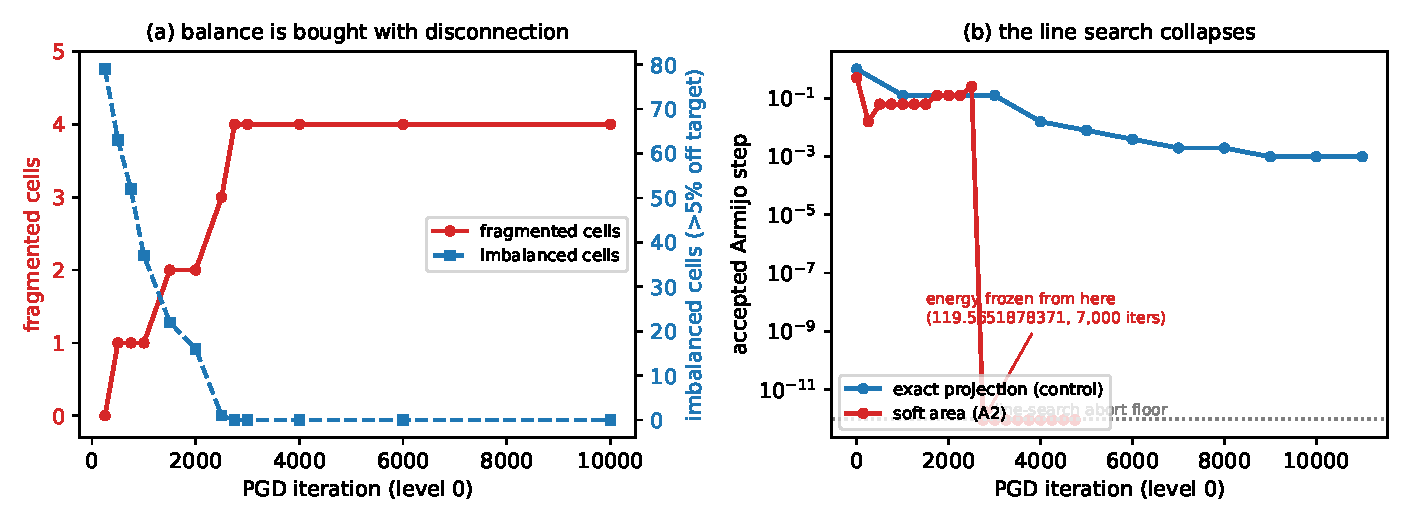
\includegraphics[width=\linewidth]{fig_two_defects.pdf}
\caption{The two independent defects. \textbf{(a)} At level~0 the
fragmented-cell count rises \(0\to4\) exactly as the imbalanced-cell count falls
\(79\to0\): the flow buys area balance with disconnected territory, and then
freezes there. \textbf{(b)} The accepted Armijo step collapses from
\(2.5\times10^{-1}\) to \(9.095\times10^{-13}\) between iterations 2{,}500 and
2{,}750 and the energy freezes to the digit, while the control's step decays
gracefully across 30{,}000 iterations and never collapses.}
\end{figure}

Fragmentation appears at iteration~500 and accumulates \emph{monotonically as
imbalance is driven out}, reaching 4 cells by iteration 2{,}750 and staying there
--- worse than the 3 the production arm ended with, so running longer makes it
worse, not better. The mechanism is in the gradient: the penalty contributes
\((\mu/\Atgt^{2})\,v_i\,(v^\top u_k - \Atgt)\), a field that is \emph{uniform
across cell \(k\)} up to the vertex weight \(v_i\). A cell short on area is
therefore boosted everywhere at once --- including wherever it holds a small
distant foothold, which grows into an island.

\paragraph{This was predicted.} \S9b of
\codefile{docs/reference/winner\_take\_all\_partition\_gap.md} was written before
A2 existed, to explain why the (rejected) discrete-area trim manufactured
islands, and it states the test: \emph{through what operator does the correction
reach the field, and is that operator local?} The trim reached the field through
the projection, a nonlocal operator. A2 reaches it through a uniform per-cell
push --- nonlocal in exactly the same sense. Two mechanisms that look nothing
alike, one criterion, one symptom. See \S\ref{sec:conclusions}.

\section{Result 3 --- defect (2): the line search collapses}
\label{sec:defect2}

The second defect is independent of the first and is the more serious one for
interpreting the headline.

\begin{center}
\begin{tabular}{@{}lrrr@{}}
\toprule
level & iterations run & step collapses at & final step \\
\midrule
A2 level 0 & 2{,}575 & 2{,}548 & \(9.095\times10^{-13}\) \\
A2 level 1 & 282 & 257 & \(9.095\times10^{-13}\) \\
A2 level 2 & 211 & 182 & \(9.095\times10^{-13}\) \\
A2 level 3 & 184 & 154 & \(9.095\times10^{-13}\) \\
A2 level 4 & 257 & 232 & \(9.095\times10^{-13}\) \\
\midrule
control level 0 & 30{,}000 & \textbf{never} & healthy \\
\bottomrule
\end{tabular}
\end{center}

\emph{Every} A2 level dies some 25--30 iterations before its ``convergence''
trigger fires. In the probe, the energy is bit-identical at
\(119.5651878371\) from iteration 2{,}750 through 9{,}999 --- seven thousand
iterations in which nothing is accepted --- with a mean of \(30.3\) backtracks
per iteration and \(11.3\%\) of wall time spent backtracking. The control never
collapses at all.

\paragraph{Why.} Once the field is crisp, the iterate sits at a vertex of the
box-truncated simplex. The Euclidean projection maps an entire small-step
neighbourhood of that point back onto the same vertex, so
\(x_{\text{trial}} = P(x - s g) = x\) exactly and \(E_{\text{trial}} = E\), while
the Armijo test demands \(E_{\text{trial}} \le E - c\,s\,\|g\|^2\) with
\(c\,s\,\|g\|^2 > 0\). No step size can satisfy it. The search backtracks
\(\sim\!40\) times to below the \(10^{-12}\) abort floor and repeats forever. The
alternating projection's multiplicative renormalisation has no such fixed point:
it keeps entries strictly positive, so small steps produce small but nonzero
motion.

\paragraph{Consequence for the headline.} A2's \(32\times\) decomposes into
\(3.1\)--\(6.4\times\) per-iteration cost and \(4.7\)--\(11.7\times\) fewer
iterations. The second factor is \emph{not a saving}: it is the optimizer dying
at every level and the energy-plateau trigger, which cannot distinguish a frozen
energy from a converged one, reporting the failure as convergence.

\begin{figure}[htbp]
\centering
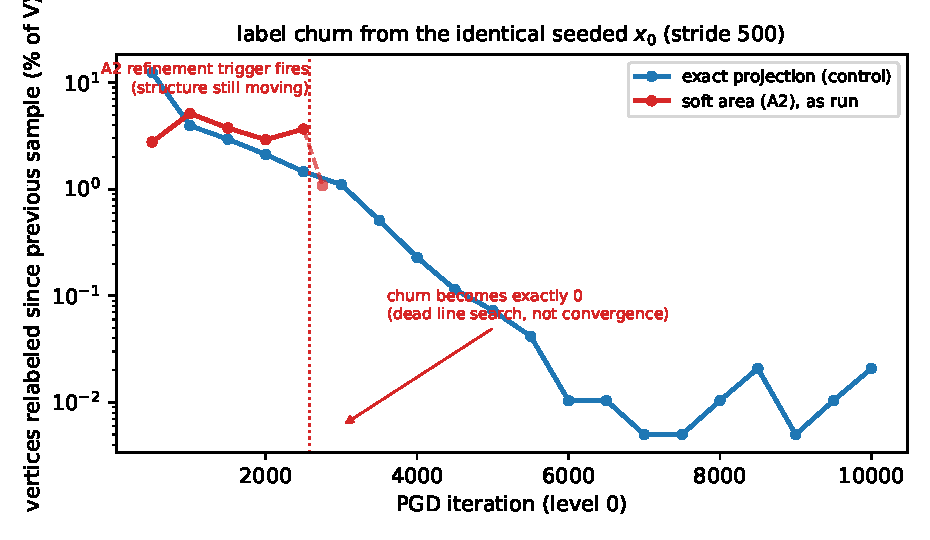
\includegraphics[width=0.78\linewidth]{fig_churn.pdf}
\caption{Winner-take-all label churn at level~0 from the identical seeded
\(x_0\). The control decays monotonically; the soft-area arm does not, and was
still relabelling \(3.7\%\) of vertices per 500 iterations when its trigger
fired at iteration 2{,}575. Past that point the churn does not become small ---
it becomes \emph{exactly} zero, for 7{,}000 iterations, which is the signature of
a dead line search rather than a settled structure.}
\end{figure}

\paragraph{A diagnostic worth stealing.} Exactly-zero churn is qualitatively
different from small churn, and it is the cheapest tell that an optimizer has
stopped rather than converged. Convergence gets \emph{cheaper} per iteration;
this got \(13\times\) more expensive per iteration at the moment it stopped
moving. A guard now warns when no step is accepted for 50 consecutive iterations
(\codefile{src/optimization/pgd\_optimizer.py}), so this failure cannot again be
mistaken for a speedup.

\section{The hybrid variant --- also closed}
\label{sec:hybrid}

One variant is not refuted by the above: run level~0 on the \emph{exact}
treatment and levels 1--4 on the soft one
(\code{soft\_area\_from\_level: 1}). Fragmentation is born at level~0
(\S\ref{sec:defect1}), and A2's finer levels never added splits beyond what
level~0 handed them, so a clean level-0 structure may survive. Both halves of the
treatment are gated together deliberately --- penalty \emph{and} projection ---
since they are separate defects and swapping only one would carry the other into
the level it was built to protect.

\paragraph{Measured (2026-08-12).} The prediction held on the mechanism and the
result is more interesting than expected.

\begin{center}
\begin{tabular}{@{}lrrr@{}}
\toprule
 & control & A2 & hybrid \\
\midrule
Phase~1 wall & \(48{,}132\)~s & \(1{,}497\)~s & \(\mathbf{7{,}044}\)~s (\(6.83\times\)) \\
level-0 line search & healthy & collapses @2{,}548 & \textbf{never collapses} \\
levels 1--4 collapse at & --- & 257/182/154/232 & 425/130/150/228 \\
dead / weak & 0 / 0 & 0 / 0 & 0 / 0 \\
imbalanced (worst) & 0 (0.78\%) & 0 (1.47\%) & 0 (1.21\%) \\
\textbf{fragmented} & \textbf{0} & \textbf{3} & \(\mathbf{0}\) \\
initial perimeter & 214.34 & 216.79 & \textbf{213.23} \\
Phase~2 & 185.2546 (20 iters) & abort @3 & \textbf{abort @1} (187.34) \\
\bottomrule
\end{tabular}
\end{center}

Two findings. First, \textbf{it confirms \S\ref{sec:defect1} directly}: making
level~0 exact removes the fragmentation entirely (\(0\) cells, no raw components
at all), so the splits really are born at level~0 and inherited, and the hybrid
passes all three validity gates at \(6.83\times\) --- better than the
\(\approx\)3.8\(\times\) predicted, because the collapsing fine levels are
\emph{cheap} as well as useless. Second, levels 1--4 collapsed exactly as
predicted (after 130--425 iterations), so they contribute almost no refinement,
and \textbf{Phase~2 still aborts} --- at iteration~1, \code{Restoration Failed!}.

That last point is not explained by anything measured here and is stated as an
open residual rather than a conclusion: the partition handed to Phase~2 is
structurally near-identical to the control's (14{,}623 variable points and 200
triple points against 14{,}641 and 200), passes all three gates, and has a
\emph{better} extracted perimeter (213.23 vs 214.34) --- yet IPOPT cannot restore
feasibility from it. Whatever Phase~2 needs from the fine levels, the three
Phase~1 validity gates do not measure it.

\paragraph{Verdict.} A valid partition at \(6.83\times\) that Phase~2 cannot
refine is not a usable pipeline, so the variant is closed with the rest of A2.
What survives is the confirmation that fragmentation is a level-0 phenomenon,
and the observation that the gates are not sufficient to certify a Phase~1
solution as Phase-2-ready.

\section{Conclusions}
\label{sec:conclusions}

\begin{enumerate}
  \item \textbf{The stated falsifier was the wrong one.} No cell died --- the
    hard mass constraint is not what keeps cells alive. A2 failed on connectivity
    and on optimizer health, neither of which was the pre-registered risk.
    Pre-registering a falsifier remains right; expecting it to be the thing that
    fires is not.
  \item \textbf{Connectivity is the fragile invariant of this problem.} Nothing
    in the energy, the constraints, or either replacement protects it. Two
    independent attempts to cheapen Phase~1 have now failed by manufacturing
    disconnected cells: the territory-aware term via nonlocal area transport
    through the projection, and A2 via a uniform per-cell push. Different
    mechanisms, identical symptom.
  \item \textbf{The locality criterion is predictive, not retrospective.} \S9b
    stated it before A2 existed and it called A2's failure mode correctly. It
    should be applied as a \emph{screening test} to any future candidate, before
    code: \emph{through what operator does the correction reach the field, and is
    that operator local?} A correction that reaches a cell uniformly, or through
    a global solve, will buy area with disconnected territory.
  \item \textbf{Do not price a speedup in iterations you did not have to run.}
    Most of the \(32\times\) was an optimizer dying early. A result that looks
    like a large speedup on a hard problem should be checked for a collapsed line
    search before it is believed.
\end{enumerate}

\section*{Related documents}
\addcontentsline{toc}{section}{Related documents}

\begin{itemize}
  \item \codefile{docs/reference/winner\_take\_all\_partition\_gap.md} --- the
    standing explanation; \S9b states the locality criterion this report
    confirms, and \S4c records the screening test.
  \item \codefile{docs/experiments/04-territory-aware-highn-validation/} --- the
    other mechanism that failed the same criterion.
  \item \codefile{docs/math/04-phase1-timing-profile/} --- the projection cost
    that motivated the attempt.
  \item Code: \codefile{src/optimization/projection.py}
    (\code{project\_rows\_onto\_simplex}),
    \codefile{src/optimization/pgd\_optimizer.py} (penalty, gate, stall guard),
    \codefile{src/partition/balanced\_readout.py} (what made the attempt
    thinkable).
\end{itemize}

\end{document}
